\section{Background}
\subsection{Economic Rationale}
\begin{frame}{Economics of Emissions Trading}
    \begin{itemize}
        \item Fix the supply $S$ of carbon in a market. \textit{Ceteris paribus}
              quantity $Q \downarrow$ and the carbon price $P \uparrow$.
        \item Increasing popularity: big markets are China ETS and EU ETS.
        \item Market price for carbon permits set through an auction.
    \end{itemize}
    \begin{figure}
        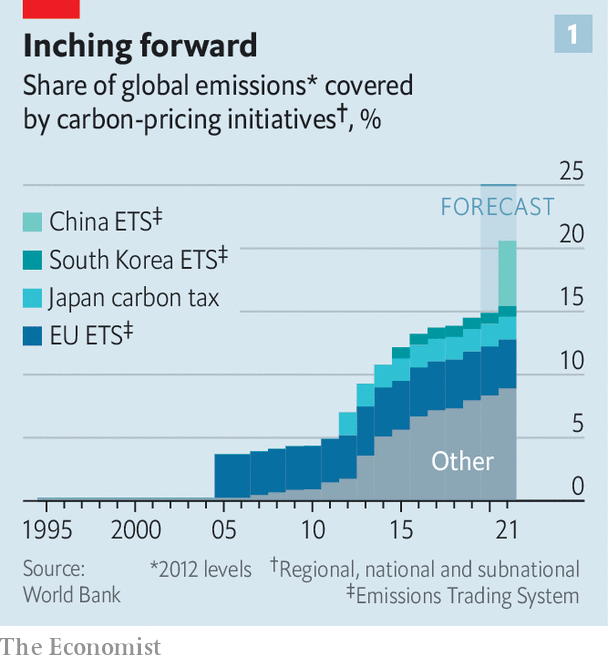
\includegraphics[height=0.5\textheight, width=\linewidth,
            keepaspectratio]{photos/ets.png}
        \centering
    \end{figure}
    \footnotetext[1]{``The World Urgently Needs To Expand Its Use Of Carbon
        Prices''. 2020. \textit{The Economist}.
        \url{https://www.economist.com/briefing/2020/05/23/the-world-urgently-needs-to-expand-its-use-of-carbon-prices}}
\end{frame}
\begin{frame}{Pricing}
    \begin{itemize}
        \item The use of \textit{smart contracts} can `nudge' consumers of
              hydrogen to use cleaner hydrogen.
              \begin{enumerate}
                  \item A `carbon price' enforced by a player in the system.
              \end{enumerate}
        \item Punishing non-clean sources of energy through smart contracts
              can accelerate the removal of negative externalities.
              \begin{enumerate}
                  \item Rapidly adjust to `cleaner' equilibria inside a market.
              \end{enumerate}
        \item Economic support: ``If economists ruled the world, carbon
              prices would drive most of the action on climate change''
              - \textit{The Economist}.
    \end{itemize}
\end{frame}
\subsection{Hydrogen Certificates}
\begin{frame}{Hydrogen Certificates}
    \begin{itemize}
        \item An approach for formally attesting the level of cleanness in
              a produced unit of hydrogen.
              \begin{enumerate}
                  \item Shared across the supply chain.
                  \item Can attest to standards related to Hydrogen
                        safety and quality.
              \end{enumerate}
        \item An agent in the blockchain can act as the certification body.
        \item Producers can \textbf{use} hydrogen certificates in the carbon
              market to spend carbon tokens.
    \end{itemize}
\end{frame}
\subsection{Existing Work in Energy Domain}
\begin{frame}{Distributed Energy System}
    \begin{itemize}
        \item \textit{Li et al., (2019)} developed a blockchain
              architecture for the energy market using smart contracts
              with non-cooperative game theory.
    \end{itemize}
    \begin{figure}
        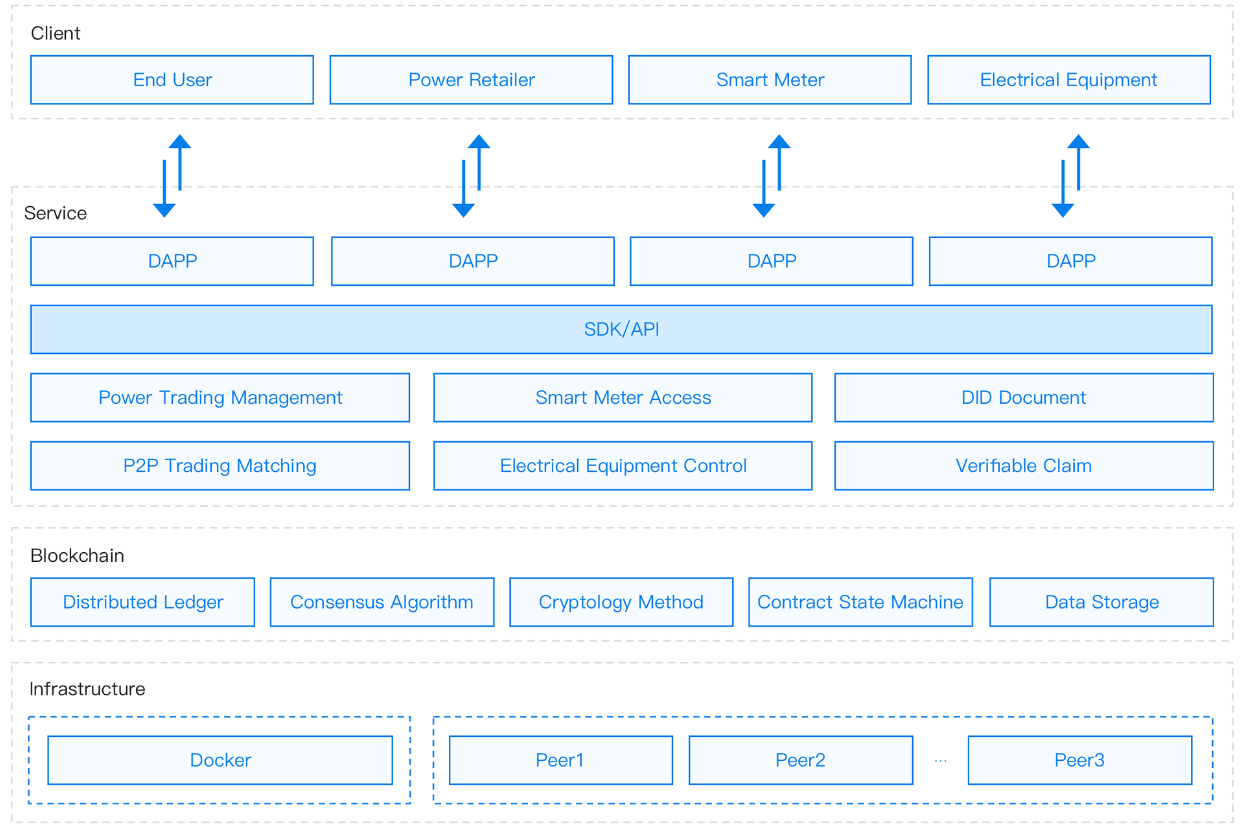
\includegraphics[height=0.5\textheight, width=\linewidth,
            keepaspectratio]{photos/blockenergy.png}
        \centering
    \end{figure}
    \footnotetext[1]{Li, Yinan, Wentao Yang, Ping He, Chang Chen,
        and Xiaonan Wang. 2019. "Design And Management Of A Distributed Hybrid
        Energy System Through Smart Contract And Blockchain".
        \textit{Applied Energy} 248:
        390-405. doi:10.1016/j.apenergy.2019.04.132.}
\end{frame}
\begin{frame}{CertifHy}
    \begin{itemize}
        \item A European certification scheme for clean hydrogen.
        \item 75,000 digital certificates issued.
        \item Software system.
        \item Allows for registration, issuing and transfer of certificates.
    \end{itemize}
    \footnotetext[1]{``Certifhy''. 2021. \textit{Certifhy.eu}.
        \url{https://www.certifhy.eu/}.}
\end{frame}
\begin{frame}{ETS for Industry 4.0}
    \begin{itemize}
        \item Khaqqi uses blockchain components to address issues with
              ETS management and fraud.
        \item Goal was to improve ETS efficiency and motivate industry
              participation.
        \item Uses a reputation system to assist with pricing.
        \item Used \textit{MultiChain} to implement.
    \end{itemize}
    \footnotetext[1]{1Khaqqi, Khamila Nurul, Janusz J. Sikorski, Kunn Hadinoto,
        and Markus Kraft. 2018. ``Incorporating
        Seller/Buyer Reputation-Based System In Blockchain-Enabled Emission
        Trading Application''. Applied
        Energy 209: 8-19. doi:10.1016/j.apenergy.2017.10.070.}
\end{frame}
\begin{frame}{TransActiveGrid}
    \begin{itemize}
        \item Blockchain and distributed generation of electricy to create a
              `point-to-point' trading model.
        \item Allowed households to sell electricity between each other.
              \begin{itemize}
                  \item Reason for the failure of the platform.
              \end{itemize}
        \item First energy market based blockchain technology in the world.
    \end{itemize}
    \footnotetext[1]{Pan, Yuting, Xiaosong Zhang, Yi Wang, Junhui Yan,
        Shuonv Zhou, Guanghua Li, and Jiexiong Bao.
        2019. ``Application Of Blockchain In Carbon Trading''.
        Energy Procedia 158: 4286-4291.
        doi:10.1016/j.egypro.2019.01.509.}
\end{frame}
\subsection{Blockchain Patterns}
\begin{frame}{Patterns}
    \begin{itemize}
        \item Token template pattern
        \item Token registry pattern
        \item Policy contract
    \end{itemize}
    \begin{figure}
        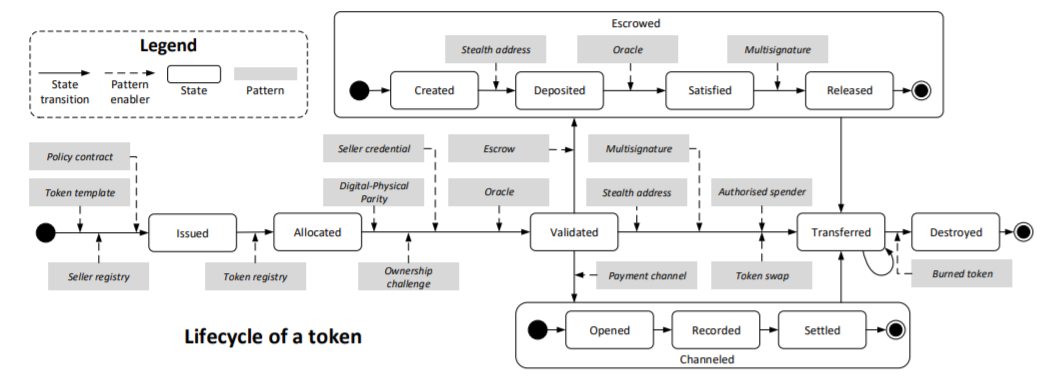
\includegraphics[height=0.5\textheight, width=\linewidth,
            keepaspectratio]{photos/token.png}
        \centering
    \end{figure}
    \footnotetext[1]{Lu, Qinghua, Xiwei Xu, Dilum Bandara, Shiping Chen,
        and Liming Zhu. 2021. \\
        ``Design Patterns For Blockchain-Based Payment Applications''.
        \textit{ACM}. doi:10.1145/1122445.1122456.\\}
\end{frame}
\begin{frame}{Token Patterns}
    \begin{itemize}
        \item Have a \textit{Carbon Coin} to represent a permit to
              emit a certain amount of carbon units (a token).
        \item \textit{Carbon Coin} is spent or `burned' on using a
              hydrogen certificate.
              \begin{itemize}
                  \item A hydrogen certificate has a level of associated carbon.
              \end{itemize}
        \item An authority handles the issuance of tokens to producers of
              carbon.
        \item Tokens are able to be purchased in auctions run by an
              authority (e.g. EU ETS).
    \end{itemize}
\end{frame}
\begin{frame}{Token Derivatives}
    \begin{itemize}
        \item To replicate a real emissions trading scheme like EU ETS,
              individuals can buy and sell derivatives of carbon tokens outside of
              a centralised authority.
        \item Financial derivatives are mappable to real tokens allowing
              producers to emit carbon.
        \item Optional trading of carbon tokens based on a `carbon reputation'
              of a buyer/seller.
    \end{itemize}
    \footnotetext[1]{Talberg, Anita, and Kai Swoboda. 2013.
        ``Emissions Trading Schemes Around The World''. Parliament
        of Australia.
        \href{https://parlinfo.aph.gov.au/parlInfo/download/library/prspub/2501441/upload_binary/2501441.pdf}
        {parlinfo.aph.gov.au}.}
\end{frame}
\begin{frame}{Policy Contract}
    \begin{itemize}
        \item Carbon tokens have policies to allow for spending.
        \item Assumption is that Hydrogen Certificates already exist in the
              system.
        \item An example policy is for carbon emissions - a certificate can be
              provided to spend carbon tokens.
              \begin{figure}
                  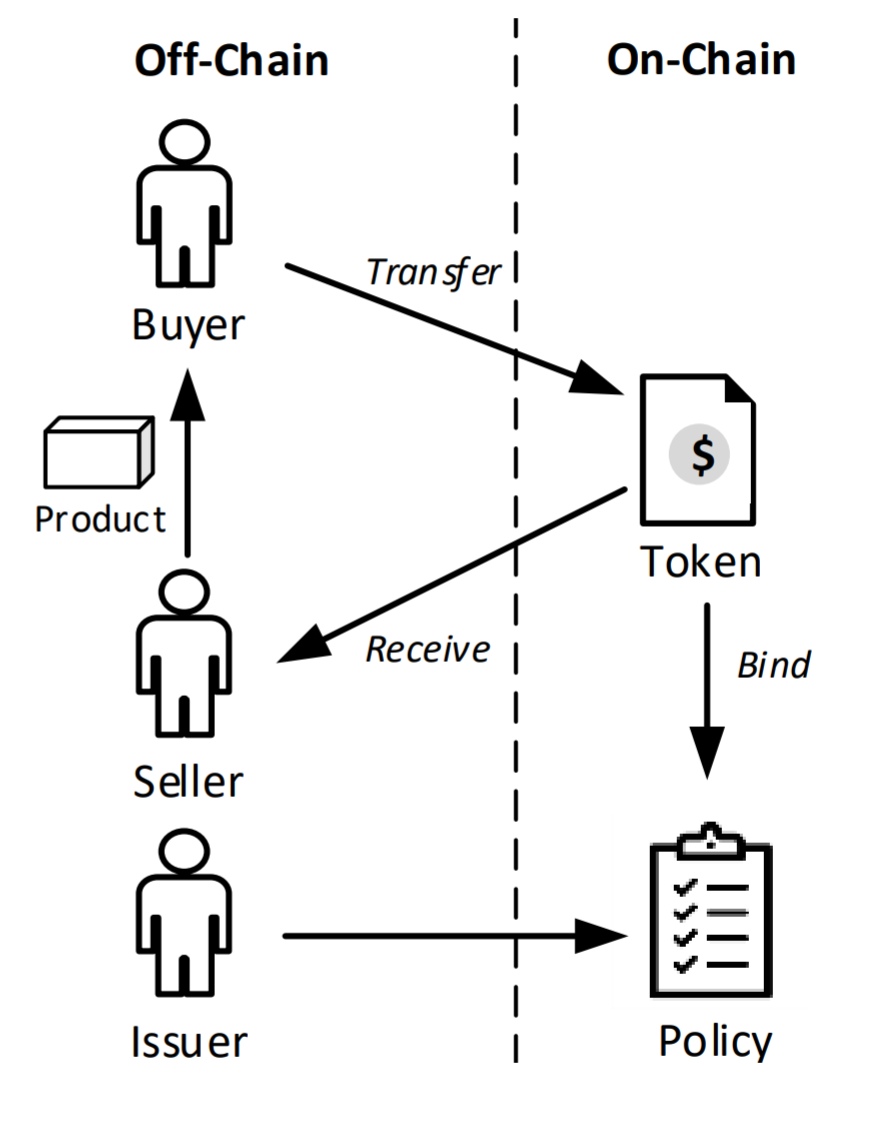
\includegraphics[height=0.4\textheight, width=\linewidth,
                      keepaspectratio]{photos/policy.png}
                  \centering
              \end{figure}
    \end{itemize}
    \footnotetext[1]{Lu, Qinghua, Xiwei Xu, Dilum Bandara, Shiping Chen,
        and Liming Zhu. 2021. \\
        ``Design Patterns For Blockchain-Based Payment Applications''.
        \textit{ACM}. doi:10.1145/1122445.1122456.\\}
\end{frame}
\subsection{Hyperledger Fabric}
\begin{frame}{Fabric}
    \begin{itemize}
        \item A modular and extensible open-source system for
              developing blockchain applications.
        \item Pluggable consensus algorithms.
        \item \textit{Chaincode} in general programming languages.
        \item Channels for enterprise confidentiality.
    \end{itemize}
    \begin{figure}
        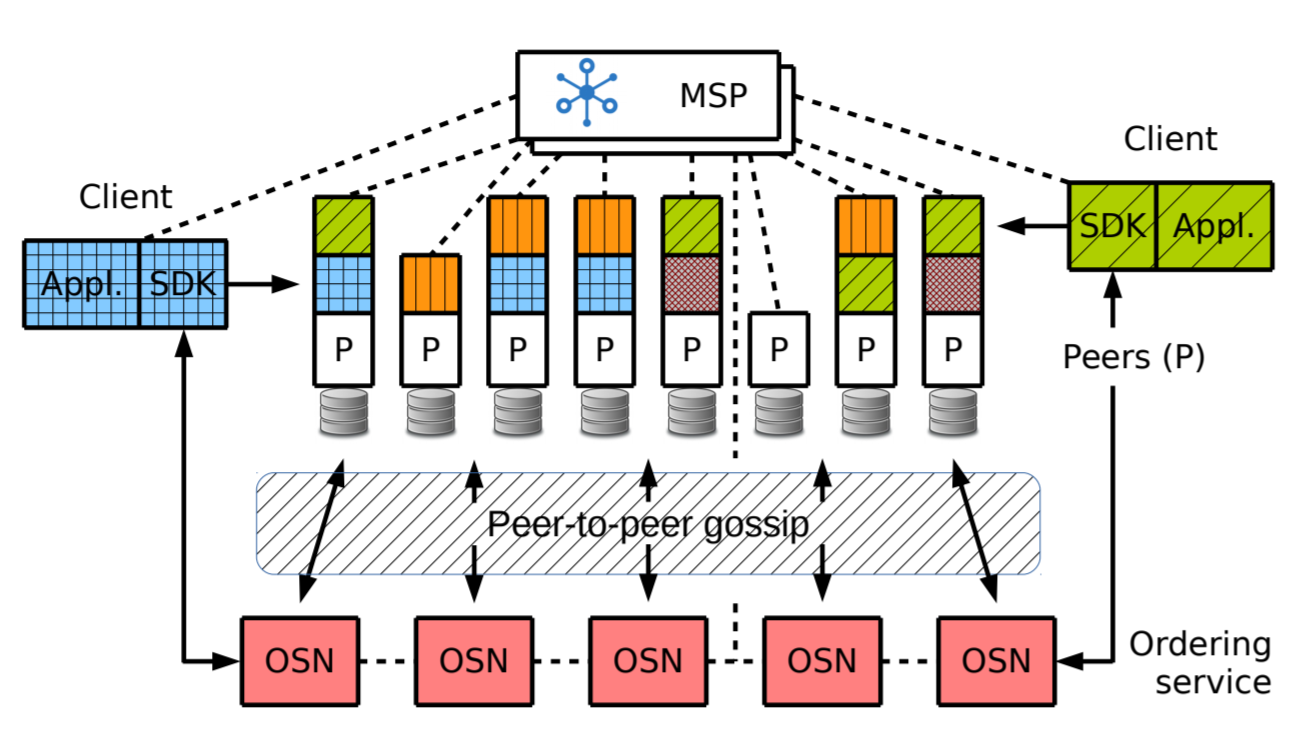
\includegraphics[height=0.4\textheight, width=\linewidth,
            keepaspectratio]{photos/fabric.png}
        \centering
    \end{figure}
    \footnotetext[1]{Androulaki, Eli, Artem Barger, Vita Bortnikov, Christian Cachin, et al.
        2018.
        ``Hyperledger Fabric: A Distributed Operating System For
        Permissioned Blockchains''.}
\end{frame}
\begin{frame}{Fabric Architecture}
    \begin{itemize}
        \item Novel \textit{execute-order-validate} architecture
              supporting high throughput transactions.
        \item Dedicated ordering nodes.
        \item Support for up to 3560 TPS (lab environment).
    \end{itemize}
    \begin{figure}
        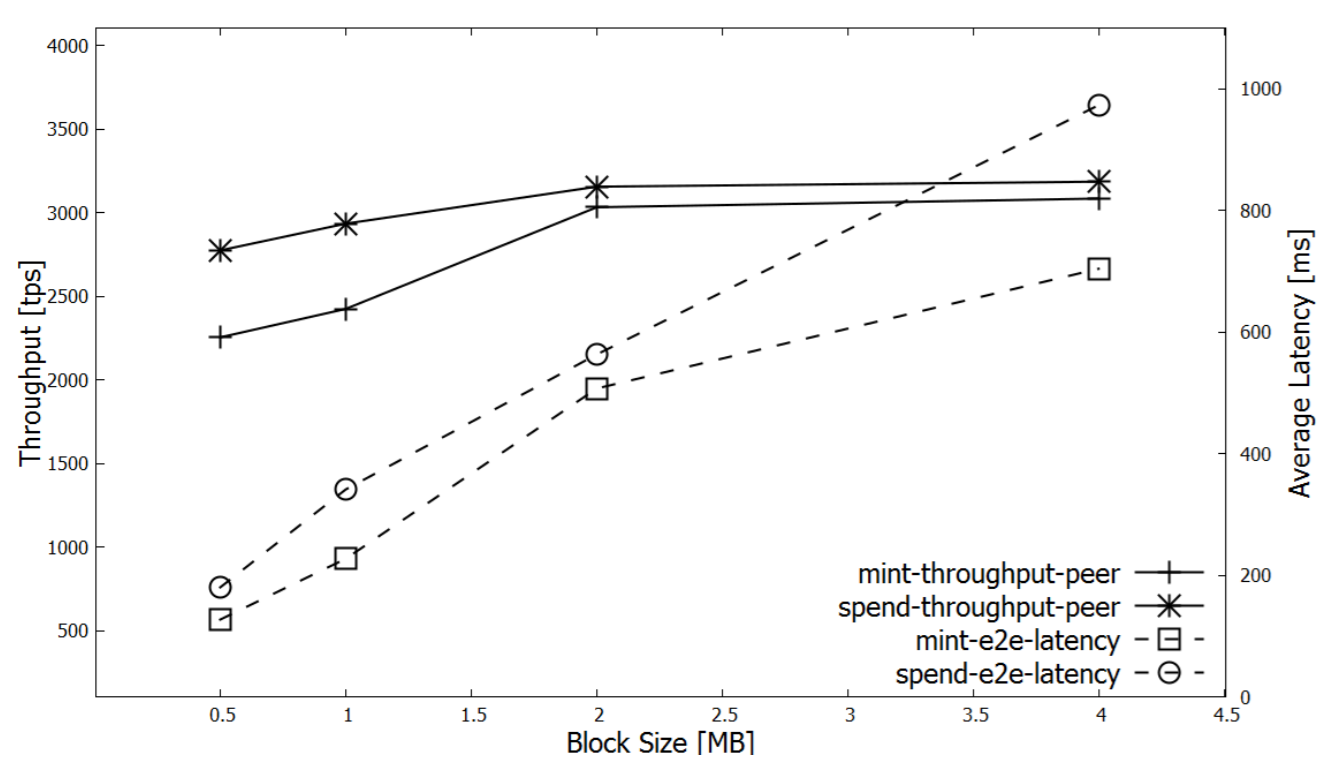
\includegraphics[height=0.4\textheight, width=\linewidth,
            keepaspectratio]{photos/tps.png}
        \centering
    \end{figure}
    \footnotetext[1]{Androulaki, Eli, Artem Barger, Vita Bortnikov, Christian Cachin, et al.
        2018.
        ``Hyperledger Fabric: A Distributed Operating System For
        Permissioned Blockchains''.}
\end{frame}
\subsection{Fabric Projects}
\begin{frame}{Fabric Projects}
    \begin{itemize}
        \item GoDirect Trade introducing trust into the supply chain for used
              aeroplane parts.
        \item OrgBook British Columbia helping small businesses find critical
              information about business partners.
        \item A permissioned blockchain as a `trust machine' for organisations.
    \end{itemize}
    \footnotetext[1]{
        ``Orgbook Case Study – Hyperledger''. 2021. \textit{Hyperledger}.
        \url{https://www.hyperledger.org/learn/publications/orgbook-case-study}.
    }
    \footnotetext[2]{
        `Case Study: Honeywell Aerospace Creates Online Parts Marketplace With
        Hyperledger Fabric'.
        2021. Blog. \textit{Case Studies}. Accessed April 14.
    }
\end{frame}
\subsection{Summary}
\begin{frame}{Summary}
    \begin{itemize}
        \item The government can use the blockchain to deliver trust and growth
              in emissions trading.
        \item Smart contracts can be applied for the buying/recording of
              emissions in a carbon market for producers.
        \item Previous blockchain energy
              solutions rely on centralised parties
              or use the blockchain to act as an `auction house'.
        \item Prior attempts disrespect user freedom by assigning a
              reputation to actors in a carbon market.
        \item Blockchain has seen recent leaps with high throughput transactions
              making the technology for a blockchain carbon market feasible.
    \end{itemize}
\end{frame}